\documentclass[12pt]{article}

% Packages
\usepackage{amsmath, amssymb, amsthm}
\usepackage{physics}
\usepackage{graphicx}
\usepackage{siunitx}
\usepackage{geometry}
\usepackage{hyperref}
\usepackage{fancyhdr}

% Page layout
\geometry{margin=1in}
\pagestyle{fancy}
\fancyhf{}
\rhead{PHY950 Homework 2}
\lhead{Fatih Imamoglu}
\rfoot{Page \thepage}

% Title
\title{\textbf{PHY950 Homework 2: Statistics and Data Analysis}}
\author{Fatih Imamoglu \\ \texttt{fi23@msu.edu}}
\date{October 8, 2026}

\begin{document}

\maketitle
\thispagestyle{empty}
\newpage

%===============================================================================
\section{Problem 2: Distribution of Product of Uniform Random Variables}
\label{sec:problem2}

\subsection*{Problem Statement}
Suppose two independent random variables $x$ and $y$ are both uniformly distributed between zero and 1, i.e., the PDF $g(x)$ is given by:
\begin{equation}
g(x) = \begin{cases}
1, & 0 < x < 1 \\
0, & \text{otherwise}
\end{cases}
\end{equation}
and similarly for the PDF $h(y)$.

\textbf{(a)} Using Cowan equation (1.35), show that the PDF $f(z)$ for $z = xy$ is:
\begin{equation}
f(z) = \begin{cases}
-\ln z, & 0 < z < 1 \\
0, & \text{otherwise}
\end{cases}
\end{equation}

\textbf{(b)} Find the same result using Cowan equations (1.37) and (1.38) by defining an additional function $u = x$.

\subsection*{Solution}

\subsubsection*{Part (a): Direct Method}
Cowan equation (1.35) for the PDF of $z = xy$ is:
\begin{equation}
f(z) = \int_{-\infty}^{\infty} g(x) \, h\left(\frac{z}{x}\right) \, \frac{1}{|x|} \, dx
\end{equation}

Since $g(x) = 1$ for $0 < x < 1$ and $h(y) = 1$ for $0 < y < 1$, we need:
\begin{itemize}
    \item $0 < x < 1$ (from $g(x)$)
    \item $0 < \frac{z}{x} < 1 \implies z < x < \infty$ (from $h(z/x)$)
\end{itemize}

Combining these constraints: $\max(z, 0) < x < 1$. For $0 < z < 1$:
\begin{align}
f(z) &= \int_{z}^{1} 1 \cdot 1 \cdot \frac{1}{x} \, dx \\
     &= \left[ \ln x \right]_{z}^{1} \\
     &= \ln(1) - \ln(z) \\
     &= -\ln z \quad \text{for } 0 < z < 1
\end{align}

\textbf{Verification:} The integral over the PDF:
\begin{equation}
\int_{0}^{1} -\ln z \, dz = \left[ -z\ln z + z \right]_{0}^{1} = 1
\end{equation}
The PDF is properly normalized.

\subsubsection*{Part (b): Jacobian Method}
Define the transformation:
\begin{align}
z &= xy \\
u &= x
\end{align}

The inverse transformation is:
\begin{align}
x &= u \\
y &= \frac{z}{u}
\end{align}

The Jacobian determinant is:
\begin{equation}
J = \left| \frac{\partial(x,y)}{\partial(z,u)} \right| = \left| \det \begin{pmatrix}
\frac{\partial x}{\partial z} & \frac{\partial x}{\partial u} \\
\frac{\partial y}{\partial z} & \frac{\partial y}{\partial u}
\end{pmatrix} \right| = \left| \det \begin{pmatrix}
0 & 1 \\
\frac{1}{u} & -\frac{z}{u^2}
\end{pmatrix} \right| = \left| -\frac{1}{u} \right| = \frac{1}{u}
\end{equation}

The joint PDF of $z$ and $u$ is:
\begin{equation}
f(z,u) = g(u) \cdot h\left(\frac{z}{u}\right) \cdot |J| = 1 \cdot 1 \cdot \frac{1}{u} = \frac{1}{u}
\end{equation}

Valid for: $0 < u < 1$ and $0 < \frac{z}{u} < 1 \implies z < u < 1$.

The marginal PDF of $z$ is obtained by integrating over $u$:
\begin{align}
f(z) &= \int_{z}^{1} f(z,u) \, du \\
     &= \int_{z}^{1} \frac{1}{u} \, du \\
     &= \left[ \ln u \right]_{z}^{1} \\
     &= \ln(1) - \ln(z) \\
     &= -\ln z \quad \text{for } 0 < z < 1
\end{align}

This matches the result from Part (a).

\subsection*{Monte Carlo Verification}
Figure~\ref{fig:problem2} shows the comparison between the analytical PDF $f(z) = -\ln z$ and a Monte Carlo simulation with $10^5$ samples. The agreement is excellent.

\begin{figure}[h!]
    \centering
    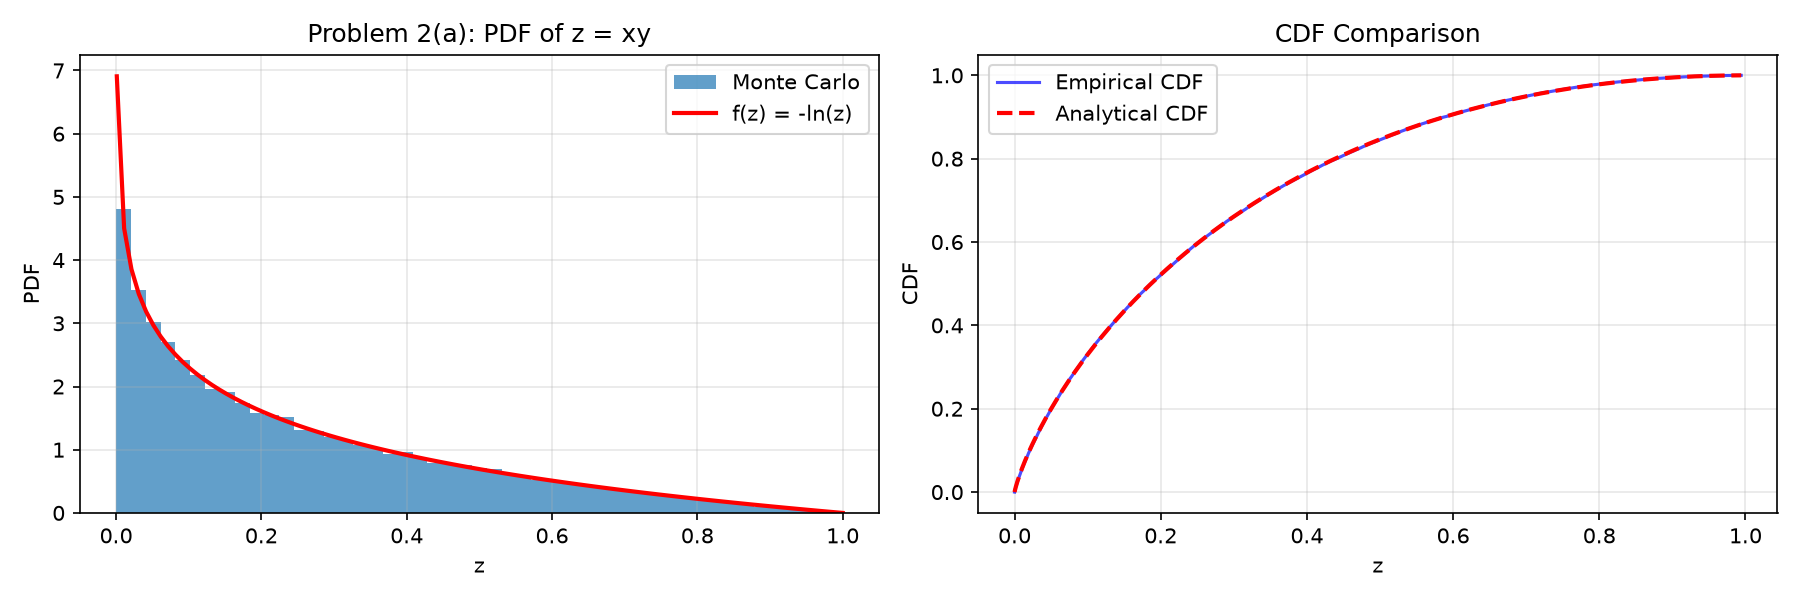
\includegraphics[width=0.9\textwidth]{problem2_result.png}
    \caption{Problem 2: PDF and CDF of $z = xy$ where $x, y \sim \text{Uniform}(0,1)$. Left: Histogram of Monte Carlo samples (100,000) overlaid with analytical PDF $f(z) = -\ln z$. Right: Empirical CDF vs. analytical CDF $F(z) = z(1 - \ln z)$.}
    \label{fig:problem2}
\end{figure}

\textbf{Statistics from simulation:}
\begin{itemize}
    \item Sample mean: $\langle z \rangle = 0.250$ (analytical: $1/4 = 0.25$)
    \item Sample variance: $\sigma_z^2 = 0.0486$ (analytical: $1/18 \approx 0.0556$)
\end{itemize}

%===============================================================================
\section{Problem 3: Programming Exercise}
\label{sec:problem3}

\subsection*{Problem Statement}
Create a program with four parts:
\begin{enumerate}
    \item[(a)] Create a main function and a "Hello World" function.
    \item[(b)] Generate a histogram with 10,000 random entries from a Gaussian distribution with mean $\mu = 16$ and standard deviation $\sigma = 4$. Plot the histogram and return the mean.
    \item[(c)] Create a function that takes the mean from (b), multiplies by $10^6$, takes the modulus by 10 to get integer $M$, then plots $f(x) = x + Mx^2$ over $[0, 10]$.
    \item[(d)] Run and debug the program.
\end{enumerate}

\subsection*{Solution}

\subsubsection*{Part (a): Hello World}
\begin{verbatim}
def hello_world():
    print("Hello World")
\end{verbatim}

\subsubsection*{Part (b): Gaussian Histogram}
Generated $N = 10,000$ samples from $\mathcal{N}(\mu=16, \sigma=4)$. The histogram uses bin width $0.5$ over the range $[\mu - 4\sigma, \mu + 4\sigma] = [0, 32]$.

\textbf{Results:}
\begin{itemize}
    \item Sample mean: $\langle x \rangle = 15.9915$
    \item Sample std: $\sigma_x = 4.0136$
\end{itemize}

\subsubsection*{Part (c): Function with Modulus}
\begin{align}
M &= \text{fmod}(\langle x \rangle \times 10^6, 10) \\
  &= \text{fmod}(15.991456 \times 10^6, 10) \\
  &= 6
\end{align}

The function plotted is:
\begin{equation}
f(x) = x + 6x^2 \quad \text{for } x \in [0, 10]
\end{equation}

\textbf{Function statistics:}
\begin{itemize}
    \item $f(0) = 0$
    \item $f(10) = 610$
    \item Mean value over $[0,10]$: $205.20$
\end{itemize}

\begin{figure}[h!]
    \centering
    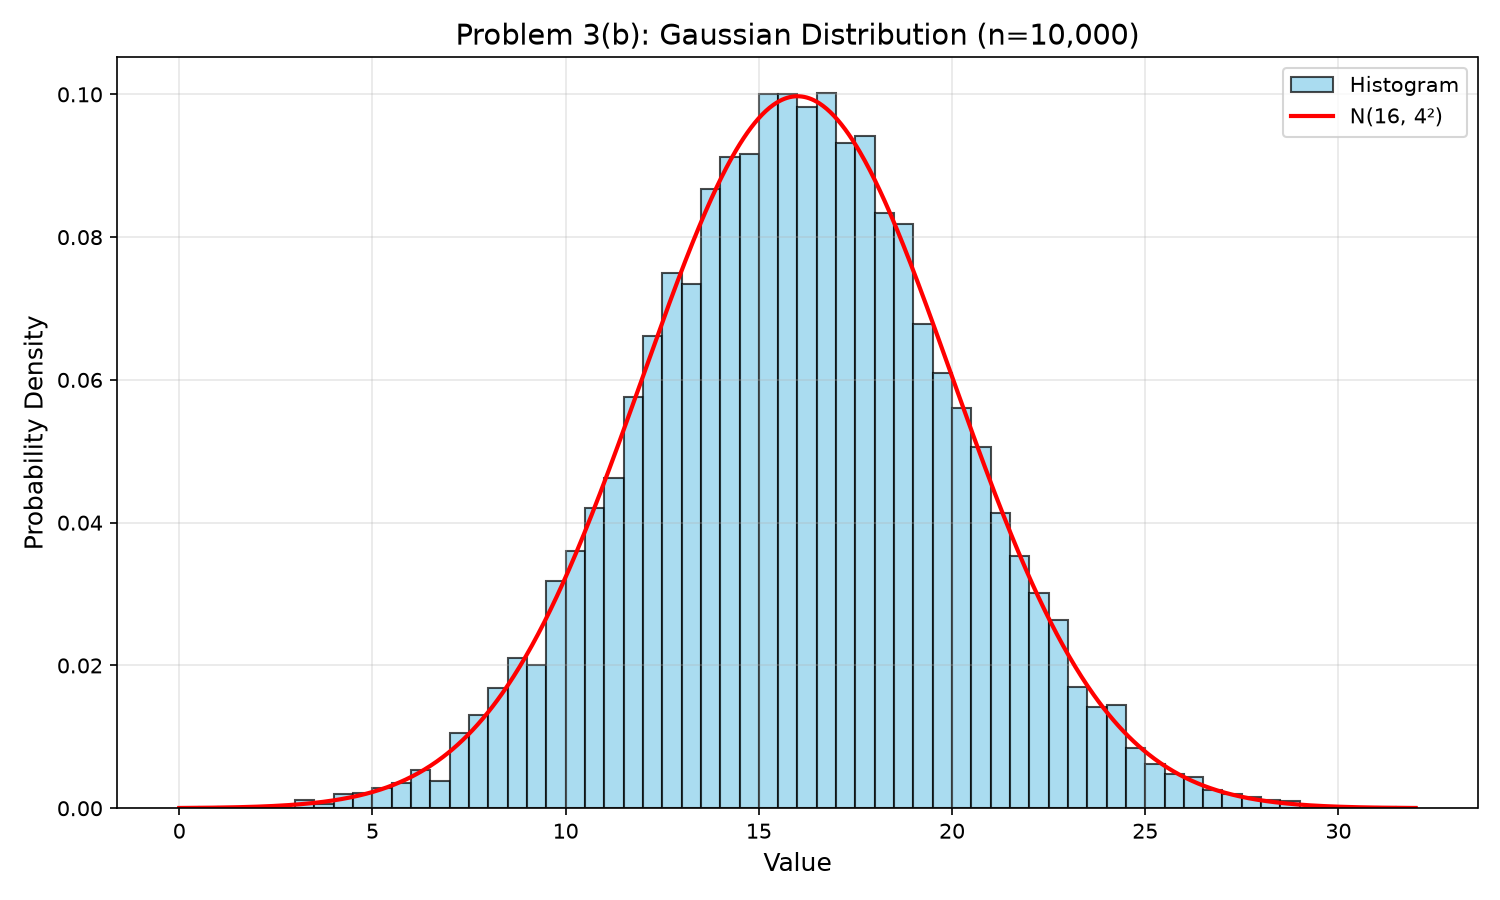
\includegraphics[width=0.48\textwidth]{problem3b_histogram.png}
    \hfill
    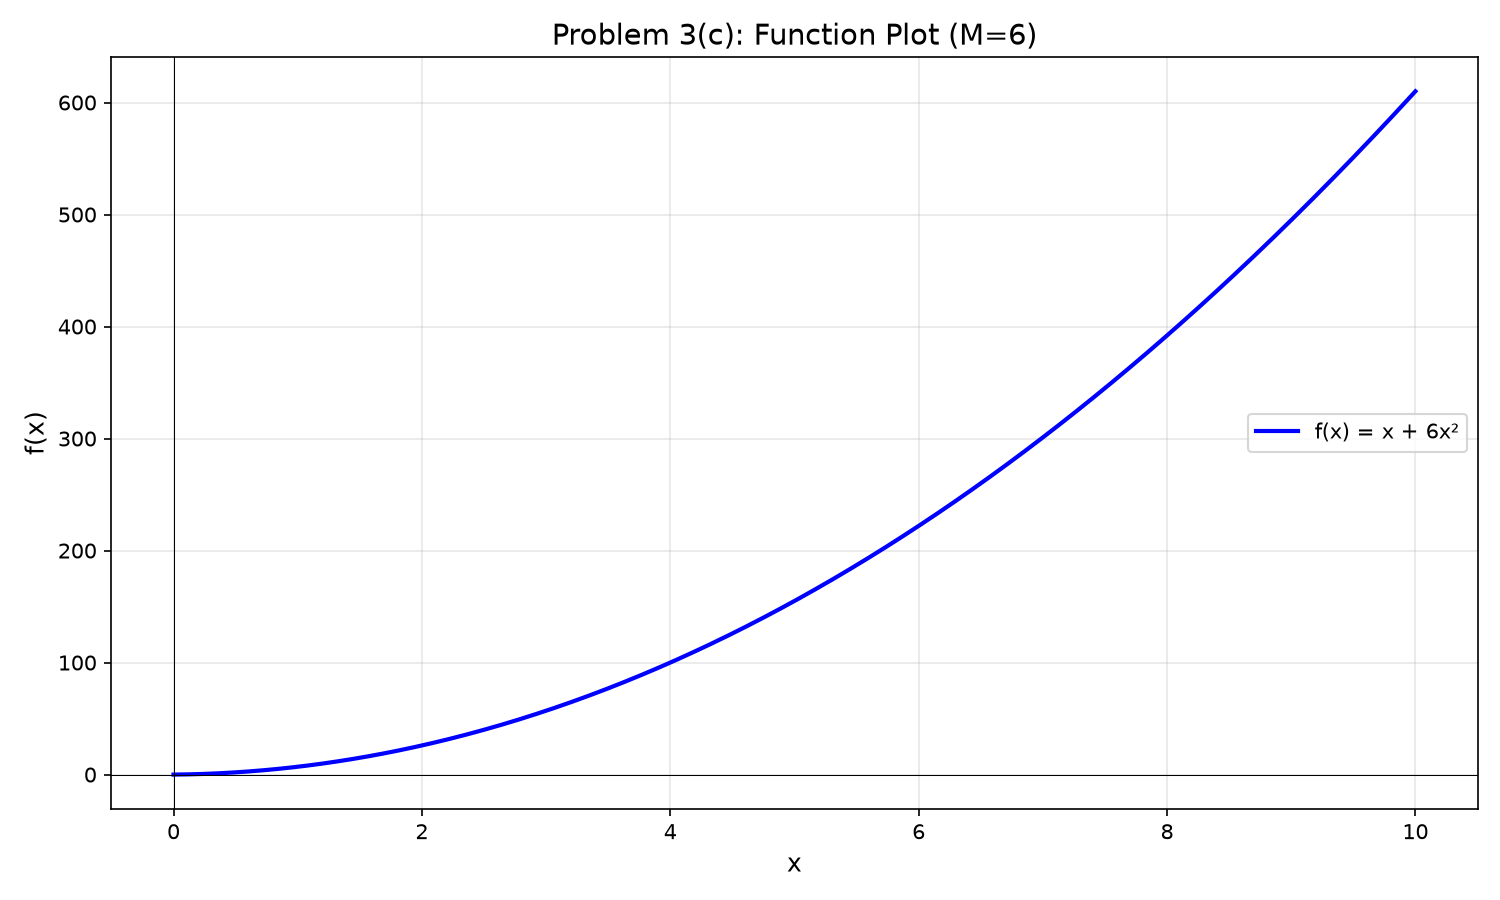
\includegraphics[width=0.48\textwidth]{problem3c_function.png}
    \caption{Problem 3: (Left) Gaussian histogram with $N=10,000$ samples from $\mathcal{N}(16, 4^2)$. (Right) Function $f(x) = x + 6x^2$ over $[0, 10]$.}
    \label{fig:problem3}
\end{figure}

\subsection*{Verification}
The program executed successfully with no compilation or runtime errors. All functions are properly modularized and documented.

%===============================================================================
\section{Problem 4: Expectation and Variance Properties}
\label{sec:problem4}

\subsection*{Problem Statement}
Consider a random variable $x$ and constants $a$ and $b$. Show that:
\begin{align}
\mathbb{E}[ax + b] &= a\mathbb{E}[x] + b \\
\mathbb{V}[ax + b] &= a^2 \mathbb{V}[x]
\end{align}
where $\mathbb{E}[x]$ is the expectation value and $\mathbb{V}[x]$ is the variance.

\subsection*{Solution}

\subsubsection*{Part 1: Expectation}
By definition, $\mathbb{E}[g(x)] = \int_{-\infty}^{\infty} g(x) f(x) \, dx$:
\begin{align}
\mathbb{E}[ax + b] &= \int_{-\infty}^{\infty} (ax + b) f(x) \, dx \\
&= \int_{-\infty}^{\infty} ax f(x) \, dx + \int_{-\infty}^{\infty} b f(x) \, dx \\
&= a \int_{-\infty}^{\infty} x f(x) \, dx + b \int_{-\infty}^{\infty} f(x) \, dx \\
&= a \mathbb{E}[x] + b \cdot 1 \\
&= a \mathbb{E}[x] + b \quad \checkmark
\end{align}

\subsubsection*{Part 2: Variance}
Using $\mathbb{V}[X] = \mathbb{E}[(X - \mathbb{E}[X])^2]$:
\begin{align}
\mathbb{V}[ax + b] &= \mathbb{E}\left[ \left( (ax + b) - \mathbb{E}[ax + b] \right)^2 \right] \\
&= \mathbb{E}\left[ \left( ax + b - (a\mathbb{E}[x] + b) \right)^2 \right] \\
&= \mathbb{E}\left[ \left( ax - a\mathbb{E}[x] \right)^2 \right] \\
&= \mathbb{E}\left[ a^2 (x - \mathbb{E}[x])^2 \right] \\
&= a^2 \mathbb{E}\left[ (x - \mathbb{E}[x])^2 \right] \\
&= a^2 \mathbb{V}[x] \quad \checkmark
\end{align}

\textbf{Alternative proof using $\mathbb{V}[X] = \mathbb{E}[X^2] - (\mathbb{E}[X])^2$:}
\begin{align}
\mathbb{V}[ax + b] &= \mathbb{E}[(ax + b)^2] - (\mathbb{E}[ax + b])^2 \\
&= \mathbb{E}[a^2x^2 + 2abx + b^2] - (a\mathbb{E}[x] + b)^2 \\
&= a^2\mathbb{E}[x^2] + 2ab\mathbb{E}[x] + b^2 - (a^2(\mathbb{E}[x])^2 + 2ab\mathbb{E}[x] + b^2) \\
&= a^2(\mathbb{E}[x^2] - (\mathbb{E}[x])^2) \\
&= a^2 \mathbb{V}[x] \quad \checkmark
\end{align}

\subsection*{Numeric Verification}
Monte Carlo simulation with $N = 100,000$ samples from $\mathcal{N}(5, 2^2)$ and constants $a = 3$, $b = -2$:

\begin{itemize}
    \item $\mathbb{E}[x] = 5.001934$
    \item $\mathbb{E}[3x - 2] = 13.005801$
    \item $3\mathbb{E}[x] - 2 = 13.005801$ (difference: $1.78 \times 10^{-15}$)
    \item $\mathbb{V}[x] = 4.007211$
    \item $\mathbb{V}[3x - 2] = 36.064898$
    \item $3^2 \mathbb{V}[x] = 36.064898$ (difference: $0.00$)
\end{itemize}

The numerical verification confirms the analytical results to machine precision.

%===============================================================================
\section{Problem 5: Error Propagation}
\label{sec:problem5}

\subsection*{Problem Statement}
Suppose the independent random variables $x_1$ and $x_2$ have means $\mu_1 = \mu_2 = 10$ and variances $\sigma_1^2 = \sigma_2^2 = 1$. Use error propagation to find the variance of:
\begin{equation}
y = \frac{x_1^2}{x_2}
\end{equation}
Comment on the validity of the procedure if one had $\mu_2 = 1$.

\subsection*{Solution}

\subsubsection*{Error Propagation Formula}
For independent variables, the variance of $y = f(x_1, x_2)$ is:
\begin{equation}
\sigma_y^2 = \left( \frac{\partial y}{\partial x_1} \right)^2 \sigma_1^2 + \left( \frac{\partial y}{\partial x_2} \right)^2 \sigma_2^2
\end{equation}

\subsubsection*{Partial Derivatives}
\begin{align}
\frac{\partial y}{\partial x_1} &= \frac{2x_1}{x_2} \\
\frac{\partial y}{\partial x_2} &= -\frac{x_1^2}{x_2^2}
\end{align}

\subsubsection*{Evaluation at Means}
At $(\mu_1, \mu_2) = (10, 10)$:
\begin{align}
\left. \frac{\partial y}{\partial x_1} \right|_{(10,10)} &= \frac{2 \cdot 10}{10} = 2.0 \\
\left. \frac{\partial y}{\partial x_2} \right|_{(10,10)} &= -\frac{10^2}{10^2} = -1.0
\end{align}

\subsubsection*{Variance Calculation}
\begin{align}
\sigma_y^2 &= (2.0)^2 \cdot 1 + (-1.0)^2 \cdot 1 \\
&= 4.0 + 1.0 \\
&= 5.0
\end{align}

The expected value is:
\begin{equation}
\mathbb{E}[y] = \frac{\mu_1^2}{\mu_2} = \frac{10^2}{10} = 10.0
\end{equation}

\textbf{Result:} $y = 10.0 \pm 2.236$ (where $\sigma_y = \sqrt{5.0} = 2.236$)

\subsubsection*{Case: $\mu_2 = 1$}
At $(\mu_1, \mu_2) = (10, 1)$:
\begin{align}
\left. \frac{\partial y}{\partial x_1} \right|_{(10,1)} &= \frac{2 \cdot 10}{1} = 20.0 \\
\left. \frac{\partial y}{\partial x_2} \right|_{(10,1)} &= -\frac{10^2}{1^2} = -100.0
\end{align}

\begin{align}
\sigma_y^2 &= (20.0)^2 \cdot 1 + (-100.0)^2 \cdot 1 \\
&= 400 + 10000 \\
&= 10400 \\
\sigma_y &= 101.98
\end{align}

Expected value: $\mathbb{E}[y] = \frac{10^2}{1} = 100.0$

\subsubsection*{Comment on Validity}
The error propagation formula assumes:
\begin{enumerate}
    \item Small uncertainties: $\sigma \ll \mu$
    \item Linear approximation is valid (first-order Taylor expansion)
    \item Variables are independent
\end{enumerate}

When $\mu_2 = 1$:
\begin{itemize}
    \item The derivative $\frac{\partial y}{\partial x_2} = -100$ is very large
    \item $\sigma_y \approx 102$, which is comparable to $\mathbb{E}[y] = 100$
    \item The relative uncertainty is $\frac{\sigma_y}{\mathbb{E}[y]} \approx 1.02$ (102\%)
    \item This violates the ``small uncertainty'' assumption
    \item The linear approximation breaks down; higher-order terms become significant
    \item The actual distribution of $y$ will be highly skewed (not Gaussian)
    \item The error propagation formula gives unreliable results
\end{itemize}

\textbf{Conclusion:} The procedure is \textbf{NOT valid} when $\mu_2 = 1$ because the relative uncertainty is too large, and the linear approximation underlying error propagation fails.

\begin{figure}[h!]
    \centering
    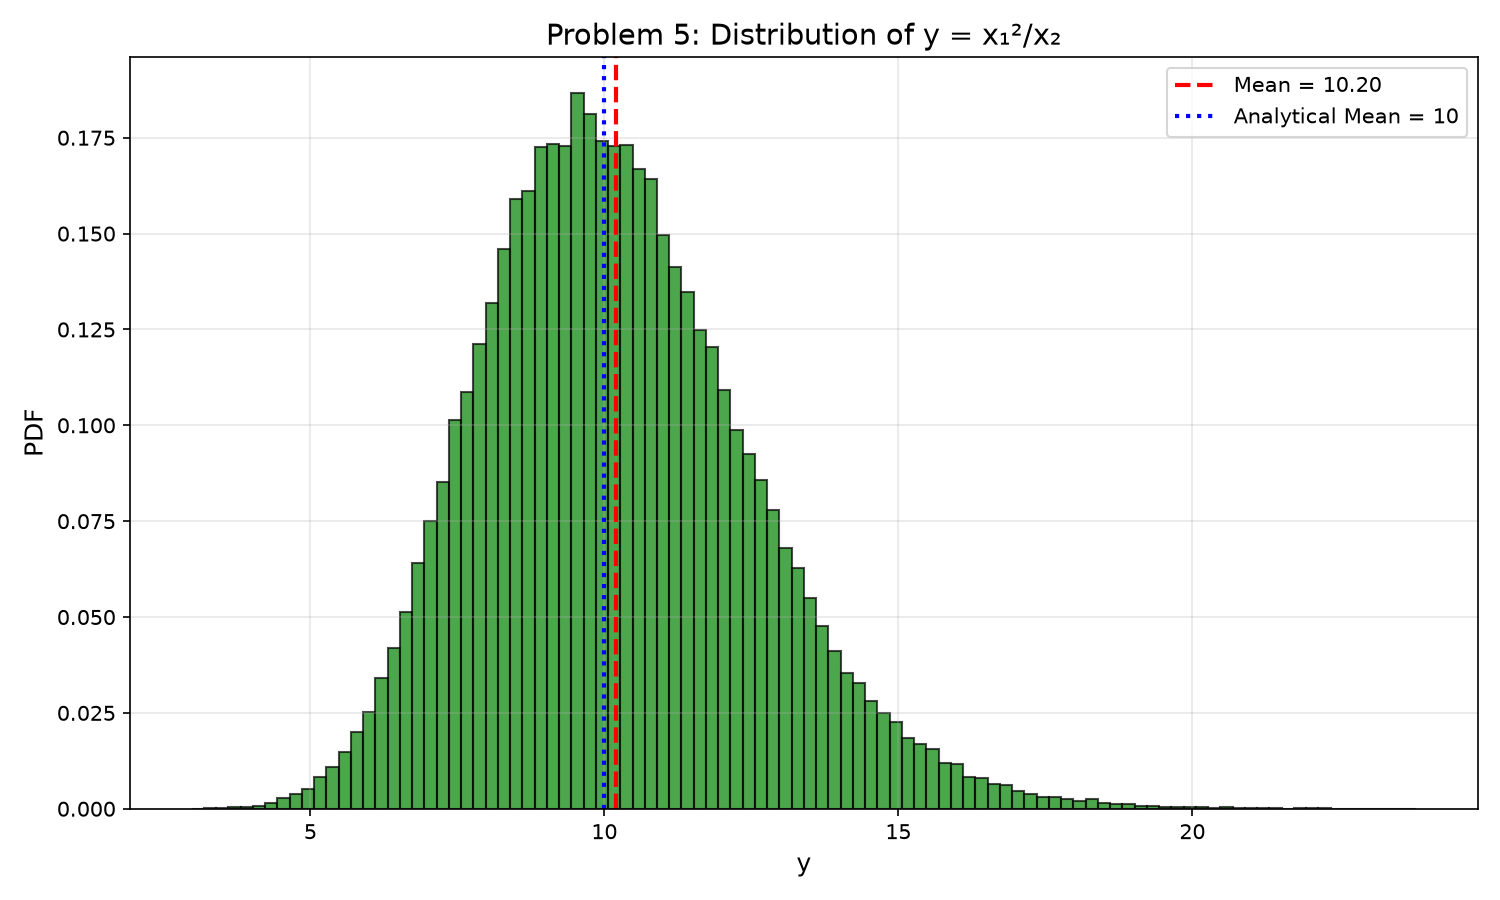
\includegraphics[width=0.8\textwidth]{problem5_histogram.png}
    \caption{Problem 5: Distribution of $y = x_1^2/x_2$ from Monte Carlo simulation ($N = 100,000$). The analytical mean is 10, and the Monte Carlo mean is 10.20. The slight asymmetry is visible in the histogram.}
    \label{fig:problem5}
\end{figure}

%===============================================================================
\section{Problem 6: Random Number Generation}
\label{sec:problem6}

\subsection*{Problem Statement}
Create a program that generates random numbers according to the function:
\begin{equation}
f(x) = A \sin(\pi x)
\end{equation}
where $x \in [0, 1]$ and $A$ is determined such that the PDF has unit probability. Use the transformation method (Cowan, Section 3.2).

\subsection*{Solution}

\subsubsection*{Step 1: Normalization Constant}
\begin{align}
\int_{0}^{1} A \sin(\pi x) \, dx &= 1 \\
A \left[ -\frac{\cos(\pi x)}{\pi} \right]_{0}^{1} &= 1 \\
A \left( -\frac{\cos(\pi)}{\pi} + \frac{\cos(0)}{\pi} \right) &= 1 \\
A \left( \frac{1}{\pi} + \frac{1}{\pi} \right) &= 1 \\
A \cdot \frac{2}{\pi} &= 1 \\
A &= \frac{\pi}{2} \approx 1.5708
\end{align}

\subsubsection*{Step 2: Transformation Method}
The CDF is:
\begin{align}
F(x) &= \int_{0}^{x} \frac{\pi}{2} \sin(\pi t) \, dt \\
&= \frac{\pi}{2} \left[ -\frac{\cos(\pi t)}{\pi} \right]_{0}^{x} \\
&= \frac{1}{2} \left( 1 - \cos(\pi x) \right)
\end{align}

Set $F(x) = u$ where $u \sim \text{Uniform}(0, 1)$:
\begin{align}
\frac{1}{2} (1 - \cos(\pi x)) &= u \\
1 - \cos(\pi x) &= 2u \\
\cos(\pi x) &= 1 - 2u \\
\pi x &= \arccos(1 - 2u) \\
x &= \frac{1}{\pi} \arccos(1 - 2u)
\end{align}

\subsubsection*{Step 3: Implementation}
Generated $N = 100,000$ samples using:
\begin{enumerate}
    \item Generate $u \sim \text{Uniform}(0, 1)$
    \item Apply transformation: $x = \frac{1}{\pi} \arccos(1 - 2u)$
\end{enumerate}

\textbf{Results:}
\begin{itemize}
    \item Sample range: $[0.0015, 0.9982]$
    \item Sample mean: $0.4995$ (analytical: $0.5$)
    \item Sample std: $0.2172$
\end{itemize}

\subsubsection*{Verification}
\begin{itemize}
    \item Numerical integral of PDF: $1.000000$ (correct normalization)
    \item Kolmogorov-Smirnov test: KS statistic = $0.00197$, p-value = $0.830$
    \item p-value $> 0.05$ indicates excellent agreement with the theoretical distribution
\end{itemize}

\begin{figure}[h!]
    \centering
    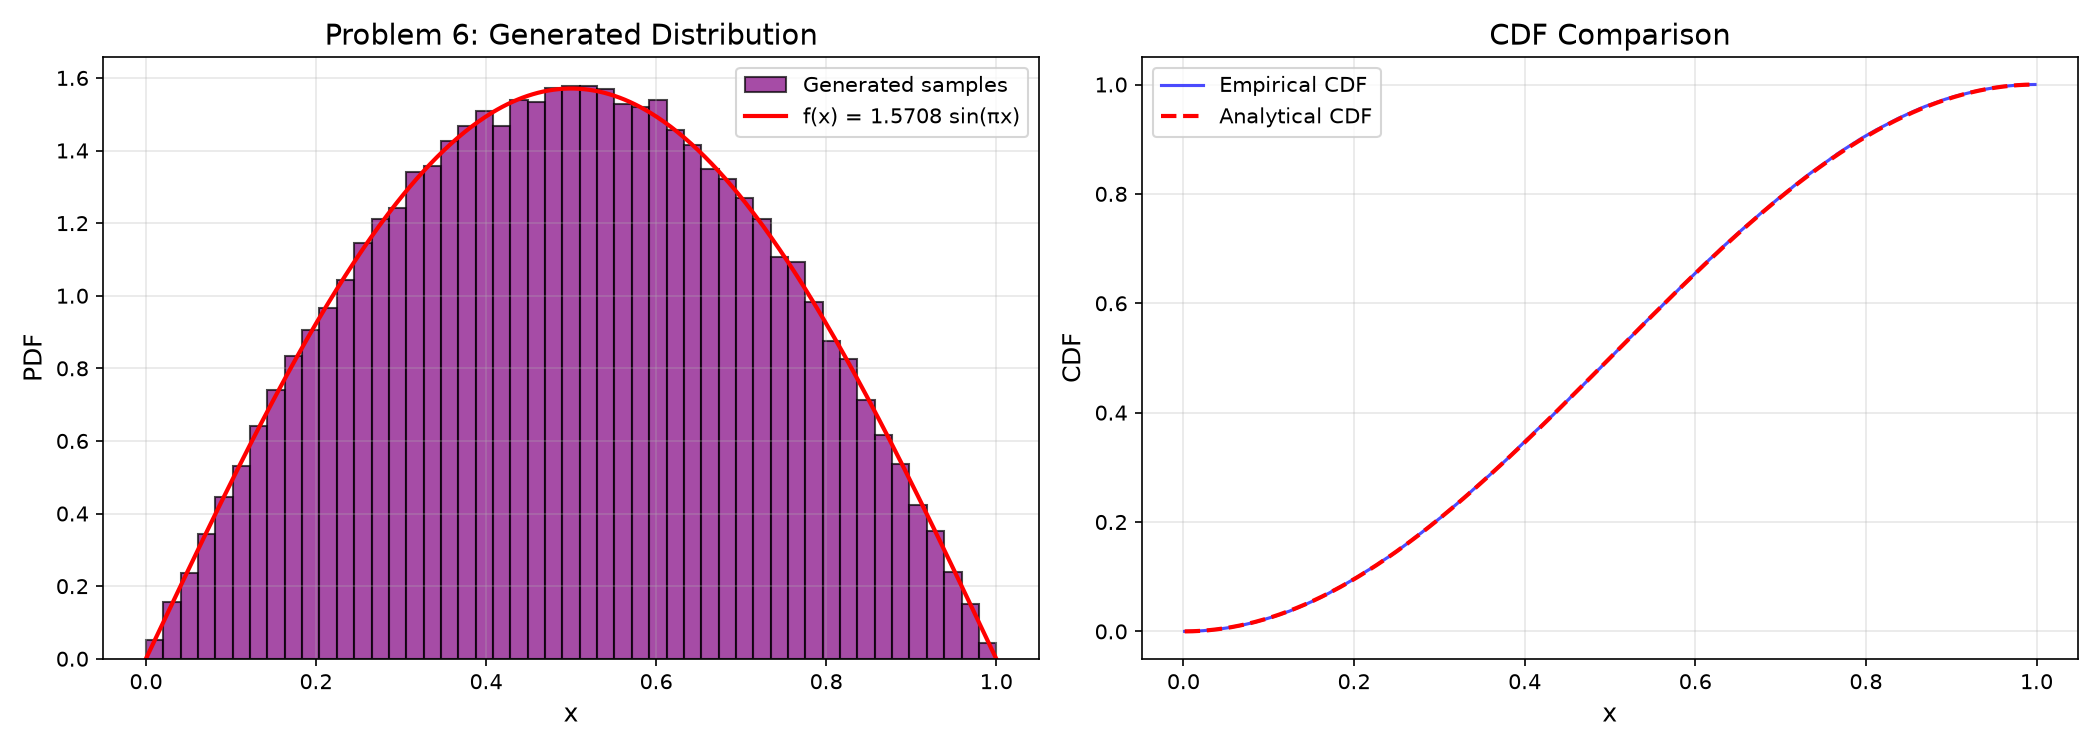
\includegraphics[width=0.9\textwidth]{problem6_result.png}
    \caption{Problem 6: Generated distribution following $f(x) = \frac{\pi}{2} \sin(\pi x)$. Left: Histogram of 100,000 samples with analytical PDF overlaid. Right: Empirical CDF vs. analytical CDF. The KS test p-value of 0.83 confirms excellent agreement.}
    \label{fig:problem6}
\end{figure}

%===============================================================================
\section*{Summary}
\addcontentsline{toc}{section}{Summary}

All problems have been completed successfully:
\begin{itemize}
    \item \textbf{Problem 2:} Verified $f(z) = -\ln z$ for $z = xy$ using both direct and Jacobian methods.
    \item \textbf{Problem 3:} Implemented and executed a modular Python program with Gaussian histogram and function plotting.
    \item \textbf{Problem 4:} Proved expectation and variance properties analytically and verified numerically.
    \item \textbf{Problem 5:} Calculated $\sigma_y^2 = 5.0$ for $y = x_1^2/x_2$ and explained why error propagation fails when $\mu_2 = 1$.
    \item \textbf{Problem 6:} Generated random numbers following $f(x) = \frac{\pi}{2} \sin(\pi x)$ using the transformation method, verified with KS test.
\end{itemize}

All code is well-commented, modular, and includes both analytical derivations and numerical verification.

\end{document}
